\section{Validation}
\label{sec:tkm:validation}

%In this paper, we propose a framework to structure and store the log of a running adaptive system in order to provide an high level API to efficiently perform diagnosis routines. 
%In this paper, we provide a novel solution to represent, manipulate, and store adaptation decisions and to trace their system states, goals, and constraints. 
This section briefly presents the implementation of our approach on top of an existing framework to store temporal graphs.
We validate our approach by first describing how one can implement graph manipulation operations involved in diagnosis algorithms. Later, we evaluate the performance of our implementation..

\subsection{Application on the smart grid example}
\label{subsec:tuto}
%\subsection{Implementation using GreyCat}
%\label{subsec:implementation}
%
%Our implementation, publicly available on GitHub\footnote{https://github.com/lmouline/LDAS}, is based on the GreyCat framework\footnote{https://github.com/datathings/greycat}: a temporal graph platform.
%The manipulated graph is defined by a set of temporal nodes and temporal edges.
%Edges are stored as references in each node.  
%The node lifetime is stored using different chunks. A chunk is created at each node modification.
%
%In addition, GreyCat comes with a lazy loading mechanism to fetch graph nodes on-demand.
%A garbage collection strategy is used to free the main memory when needed.
%This strategy is implemented using a counter on each node. This counter increases or decreases with the number of references to the node. When this counter is equal to zero,  the node is explicitly released by calling a \textit{free} method.
%
%Thanks to the GreyCat graph framework, we are able to define a metamodel with time as a built-in concept. The metamodel defines typed nodes and labeled edges. In our implementation we mapped all presented classes (Figures~\ref{fig:context-model}~-~\ref{fig:knowledge-mm}) to a GreyCat class. Based on this metamodel, a set of Java classes is created. These classes define attributed and method to manipulate a knowledge model (creation, modification, reading, and suppression). We define our navigation API on top of Greycat's Task API\footnote{https://greycat.ai/doc/tasks/}, a Gremlin-like graph traversal language\footnote{https://tinkerpop.apache.org/gremlin.html}. Greycat's Task API is a fluent API that defines a set of actions to manipulate and traverse the graph.%
To validate and evaluate our approach, we implemented a prototype publicly available online~\footnote{https://github.com/lmouline/LDAS}.
This implementation leverages the GreyCat framework\footnote{https://github.com/datathings/greycat}, more precisely the modeling plugin, which allows designing a metamodel using a textual syntax. Based on this specification, GreyCat generates a Java and a JavaScript API to create and manipulate models that conform to the predefined metamodel. The GreyCat framework handles time as a built-in concept. Additionally, it has a native support of a lazy loading mechanism and an advanced garbage collection. This is achieved by dynamically loading and unloading model elements from the main memory when necessary.

In what follows, we explain how a stakeholder, Morgan, can apply our approach to a smart grid system in order to, first, abstract adaptive system concepts, then, structure runtime data, and finally, query the model for diagnosis purpose.
The corresponding object model is depicted in Figure~\ref{fig:action-om}.
Due to space limitation, we only present an excerpt of the knowledge model.
An elaborate version is accessible in the tool repository.\looseness=-1

\paragraph{\textbf{Abstracting the adaptive system}}

At design time ($t_d$), either manually or using an automatic process, Morgan abstracts the different tactics and actions available in the adaptation process.
% Note the precise semantics of the action is not stored in the model, only an identifier (\eg the name of the action) is used to make the links.
Among the different tactics that Morgan would like to model is  ``\textit{reduce amps limit}". 
It is composed of three actions: sending a request to the smart meter (\textit{askReduce}), checking if the new limit corresponds to the desired one (\textit{checkNewLimit}), and notifying the user by e-mail (\textit{notifyUser}). 
Morgan assumes that the \textit{askReduce} action impacts consumption data (\textit{csmpt}).
This tactic is triggered upon a query (\textit{tempQ}) that uses meter (\textit{mt}), consumption (\textit{csmpt}) and customer (\textit{cust}) data. The query implements the ``\textit{no overload}" goal: the system shall never have a cable overload. 
Figure~\ref{fig:action-om} depicts a flattened version of the temporal model representing these elements. The tag at upper-left corner of every object illustrates the creation timestamp. All the elements created at this stage are tagged with $t_d$.

\paragraph{\textbf{Adding runtime information}}
%At runtime, the adaptation process will analyze the context and may trigger the previously described action. For each performed \textit{execution} a corresponding data element is created and stored, and links to context values involved in the adaptation process are set up. A decision element is also created to represent the made decision and links to actions execution are built to represent its circumstances. 
%The model will mainly store the following information of the executions: starting time, end time, modification times and the status.

%Let us suppose that at $t_0$, the adaptation process started in parallel two executions of the previously described tactic, starting with the action named \textit{askReduce}.
%At $t_1$, the second action succeeded and triggered, in parallel, the action \textit{checkNewLimit} and \textit{notifyUser}, which finished at $t_6$ and $t_3$ respectively.
%All the actions were created at $t_0$, thus, forming the execution plan of the tactic. The property \textit{status} provides information about the execution stage of each action. Figure~\ref{fig:action-om} depicts the system state, queried at $t_2$. As you can notice, only $t_2$
%
%%that finishes at $t_6$ and \textit{notifyUser} that finished at $t_3$.
%At $t_2$, the first action \textit{askReduce}, will also succeed.
%Then, \textit{checkNewLimit} is executed until $t_5$ and \textit{notifyUser} until $t_4$.
%Figure~\ref{fig:action-om}, we depict the object model, queried at $t_2$. 
%Querying it at another time will change the status of the different executions.

The adaptation process checks if the current system state fulfills the requirements by analyzing the context. To perform this, it executes the different temporal queries, including \textit{tempQ}.
For some reasons, the {tempQ} reveals that the current context does not respect the ``\textit{no overload}" goal. To adapt the smart grid system, the adaptation process decides to start the execution of the previously described tactic (\textit{exec1}) at $t_s$. As a result,  
a decision element is added to the model along with a relationship to the unsatisfied goal. In addition, this decision entails the planning of a tactic execution, manifested in the creation of the element \textit{exec1}and its subsequent actions (\textit{notifyU}, \textit{checkLmt}, and \textit{askRed}). At $t_s$, all the actions execution have an IDLE status and an expected start time. All the elements created at this stage are tagged with the $t_s$ timestamp in Figure~\ref{fig:action-om}.\looseness-1

At $t_{s+1}$, the planned tactic starts being executed by running the action \textit{askReduce}. The status of this action turns from \textit{IDLE} to \textit{RUNNING}. Later, at $t_{s+2}$, the execution of \textit{askReduce} finishes with a \textit{SUCCEED} status and triggers the execution of the actions \textit{notifyUser} and \textit{checkNewLimit} in parallel. The status of \textit{askReduce} changes to \textit{SUCCEED} while the status of \textit{notifyUser} and \textit{checkNewLimit} turns to \textit{RUNNING}.
The first action successfully ends at $t_{s+3}$ while the second ends at $t_{s+4}$. As all actions terminates with a \textit{SUCCEED} status at $t_{s+4}$, accordingly, the final status of the tactic is set \textit{SUCCEED} and the \textit{stop} attribute value is set to $t_{e}$.  

% At $t_e$, a new consumption value is measured. 
% As it already exists a valid value at this timestamp (\textit{ve1}), the measured value should have been impacted by the previous decision.
% We then overwrite the value of the previously created element by the new one. The context used by the query as well as the impacted values are also linked to this newly created element, respectively, through the \textit{inputValues} and the \textit{impactValues} relationships

%During the execution of the tactic \textit{exec1}, for every action execution, a corresponding node is created and its status is updated. At $t_e$, when the planned tactic execution finished, the context model is updated and links to the impacted context are created. 


 %Let us suppose that at $t_0$ the adaptation process started an execution of the previously described tactic, starting with the action named \textit{askReduce}.
%This action finished at $t0$ with a \textit{SUCCEED} status and triggered the execution of the action \textit{notifyUser} and \textit{checkNewLimit} in parallel.
%The first one successfully ended at $t_4$ and the second one at $t_5$.
%As all actions have terminated with a \textit{SUCCEED} status at $t_5$, the final status of the tactic is also \textit{SUCCEED} and the \textit{stop} property is set at $t_5$.
%
%This tactic has been executed because the execution of temporal query revealed that the context, \it the input context, did not respect the ``\textit{no overload}" goal.
%Its execution should impact the consumption (structure named \textit{Consumption}) and meter information (structure named \textit{meter})

\begin{figure*}
	\centering
	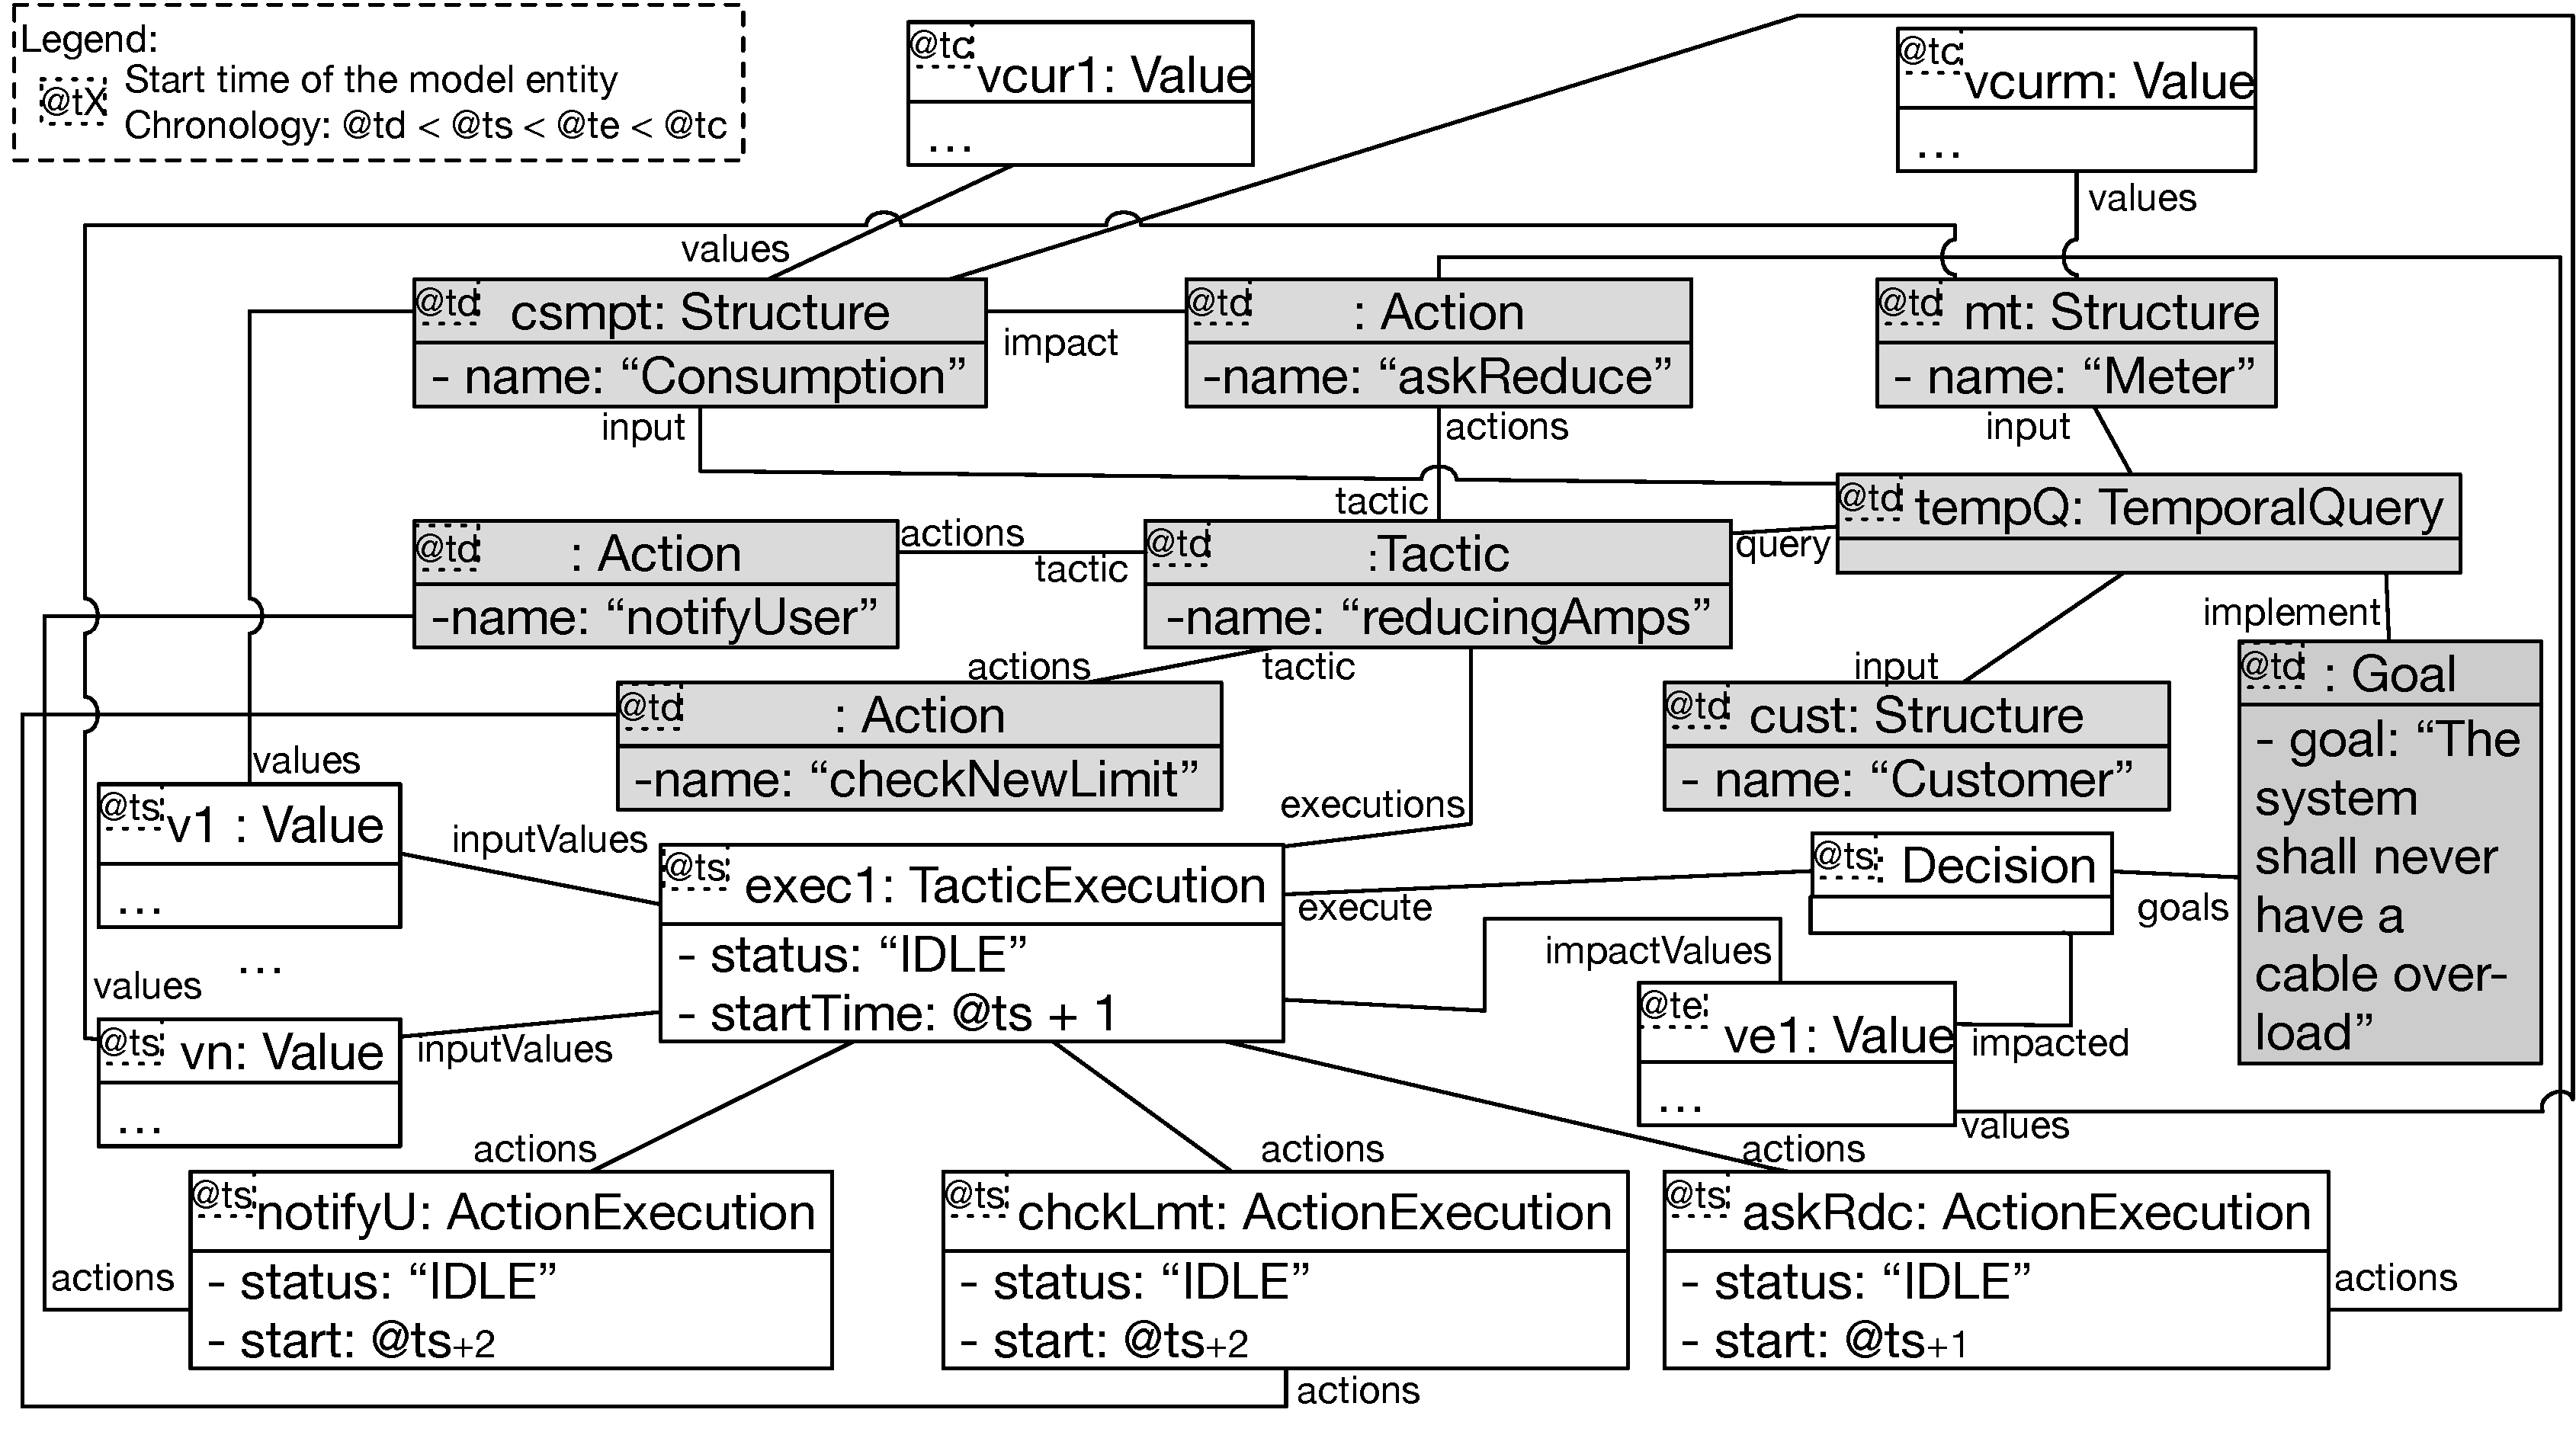
\includegraphics[width=.6\linewidth]{img/chapt-tkm/validation/action-om}
	\caption{Excerpt of the knowledge object model related to our smart grid example}
	\label{fig:action-om}
\end{figure*}

\paragraph{\textbf{Interactive diagnosis query}}

%Using the aforementioned action model, Morgan would be able to query the system state and understand why it has executed these actions and what were the expected impacts.
%In other words, she/he can diagnose the system by getting the decisions and their circumstances.
%As described in Section~\ref{sec:example}, among the questions that Morgan would like to try to answer is: What goal(s) the system was trying to reach and what were the input values that the adaptation process used when it reduced the power consumption of the customer C?
%
%Considering that the reduction of the amps limit of customer C is made was impacted by the first execution of the described tactic, answering this question results in navigating through the \textit{TacticExecution.inputValues}  and the \textit{TacticExecution.decision.goals}. \ab{Usually the user does not know what execution impacted a subpart of the context... Perhaps we should consider adding a query discovering the responsible execution first.}
%Using our implementation, this query can be described as follows:

%At $t_7$, a customer complains about a lot of cut off for a couple of days.
%The system may be in a suboptimal state.
%As described in Section~\ref{sec:example}, she/he will try to answer the following questions: did the system make any decision(s) that could have impacted the customer consumption? 
%If so, what goal(s) the system was trying to reach and what were the values used at the time the decision(s) was(were) made?


%The starting point of this function is the current (at $t_7$) consumption value, depicted by one of the value objects on the left side of the Figure~\ref{fig:action-om}.
%The first step if to get all previous data that have been measured for the past two days.

After receiving incident reports concerning regular power cuts, and based on the aforementioned knowledge model, Morgan would be able to query the system's states and investigate why such incidents have occurred.
As described in Section~\ref{sec:example}, she/he will interactively diagnose the system by interrogating the context, the decisions made, and their circumstances.

The first function, depicted in Listing~\ref{code:actions-to-goals}, allows  to navigate from the currently measured values (\textit{vcur1}) to the decision(s) made. The for-loop and the if-condition are responsible for resolving the measured data for the past two days. 
Past elements are accessed using the \textit{resolve} function that implements the $\mathcal{Z}^T$ relation (\cf Section~\ref{sec:formalism}).
After extracting the decisions leading to power cuts, Morgan carries on with the diagnosis by accessing the circumstances of this decision. The code to perform this task is depicted in Listing~\ref{code:actions-to-goals}, the second function (getCircumstances).
Note that the relationship \textit{Decision.input} is the aggregation of \textit{Decision.excecute.inputValues}.

\begin{lstlisting}[style=customc,caption=Get the goals used by the adaptation process from executed actions, label=code:actions-to-goals,basicstyle=\scriptsize]
// extracting the decisions
Decision[] impactedBy(Value v) {
  Decision[] respD
  for( Time t: v.modificationTimes() ):
    if (t >= v.startTime() - 2 day)
      Value resV = resolve(v,t)
    respD.addAll(from(resV).navigate(Value.impacted))
  return respD
}
// extracting the circumstances of the made decisions
Tuple<Value[], Goal[]> getCircumstance(Decision d) {
  Value[] resValues = from(d).navigate(Decision.input)
  Goal[] resGoals = from(d).navigate(Decision.goals)      
  return Tuple<>(resValues, resGoals)
} 
\end{lstlisting}

%%% CAN BE USED TO WIN 3 LINES                    %%%
%%% TEXT SHOULD BE ADAPTED IF WE USE IT %%%
%\begin{lstlisting}[style=customc,caption=Get the goals used by the adaptation process from executed actions, label=code:actions-to-goals,basicstyle=\scriptsize]
%Tuple<Decision[],Value[], Goal[]> diagnose(Value v) {
%  Decision[] respD
%  for( Time t: v.modificationTimes() ):
%    if (t >= v.startTime() - 2 day)
%      Value resV = resolve(v,t)
%      respD.addAll(from(resV).navigate(Value.impacted))
%      
%  Value[] resValues = from(respD).navigate(Decision.input)
%  Goal[] resGoals = from(d).navigate(Decision.goals)      
%  return Tuple<>(return respD, resValues, resGoals)
%} 
%\end{lstlisting}

%\subsection{Diagnosis validation}
%Below, we depict code excerpts of some diagnosis routines. 
% In particular, show how the questions defined in Section~\ref{sec:introduction-motivation} can be described using our implementation.
%The navigation API uses a dot notation to access the graph properties (attributes and relationships). Elements are considered as a stream, similar to Stream Java interface\footnote{https://docs.oracle.com/javase/8/docs/api/java/util/stream/Stream.html, Last visited: 28 September 2017}.
%%The execution semantics also remains similar.
%To simplify the presented code, we define a function \textit{resolve} that takes a node and a time (or a set of nodes and a set of times) and returns the state of the node(s) at the given time(s): $resolve(node, time) \rightarrow node[time]$.
%Navigation operations are executed at the timestamp of the first node element. For instance, the expression \textit{class.children.att1} navigates throw the \textit{children} relation from class \textit{class}, resolves the targeted node(s) at the time \textit{t} and reads the value of the attribute \textit{att1}: \textit{class[t].children[t].att1[t]}.
%
%\paragraph{What goal(s) the system was trying to reach by executing a tactic $a$?}
%Tracing back from a malicious behavior to the goals it was trying to reach is an important question the developers try to answer when localizing faults.
%In Listing~\ref{code:actions-to-goals}, we show a pseudo-code example of a function that given a temporal node and a timestamp returns the set of goals the system was trying to reach.  
%
%
%\begin{lstlisting}[style=customc,caption=Get the goals used by the adaptation process from executed actions, label=code:actions-to-goals,basicstyle=\scriptsize]
%function getGoals(a: Action[], t: Time[]): Goal[] {
%  Action[] timedA = resolve(a,t)
%  return timedA.tactic.condition.goals
%} 
%\end{lstlisting}
%
%This algorithm can be used to answer the first question of our use case example: what goal(s) the system was trying to reach by cutting off the power consumption of the building B?
%As "cutting off the power" will be stored by a node that conforms to the Action metaclass, it will possess an edge to a node that stores its tactic.
%This node will have an edge to another one that represents the condition and finally an edge to the node that stores the condition.
%
%\paragraph{What were the circumstances used by a decision $d$ and its expected impact on the context?}
%Decisions are made by applying the requirements in a precise context.
%When decisions result in a suboptimal state, it is important to know what were the context state and the requirements that the system was trying to satisfy at this moment.
%In Listing~\ref{code:decision-to-goals}, we show how we can navigate from a decision to its goals and its input and impacted context.
%
%\begin{lstlisting}[style=customc,caption=Get the context and the goals of a precise decision,label=code:decision-to-goals,basicstyle=\scriptsize]
%function getCircumstancesAndImpact(d: Decision):
%                           Tuple<Values[], Goals[], Values[]> {
%  return new Tuple(d.input, d.goals, d.impact)
%}
%\end{lstlisting}
%
%An engineer can apply this algorithm to extract the data for the next two questions: when the system has decided to reduce the power consumption of M. and Ms. X, what was the load of the network of their districts and when the system has decided to connect the production unit, what was the expected network load?
%However, the algorithm extracts both circumstances and impact at the same time.
%Here, there are two nodes that conform to the \textit{Decision} metaclass: one for the reduction of the power consumption and another one for the connection of a production unit.
%Following the same reasoning as made for the previous code, by navigating to the relationships defined in the metaclass, the algorithm will be able to traverse the elements until the goals or the impacted elements.
%
%\paragraph{What decision(s) influenced the system's context at a time $t$?}
%Context at a precise timestamp may be influenced by decisions made earlier.
%In order to understand how the context results in a suboptimal configuration, not only the modification of the environment should be understood but also the decisions made.
%In Listing~\ref{code:context-to-decision}, we show how we can get the decisions made that have expected values, \ie expected impacted, in the context at a given time.
%
%\begin{lstlisting}[style=customc,caption=Get decisions that may have impacted the context,label=code:context-to-decision,basicstyle=\scriptsize]
%function getDecisions(c: Context, t: Time): Decisions[] {
%  Context timedC = resolve(c,t)
%  Decisions[] resultD = Decisions[]
%
%  resultD.add(timeC.structures.properties.expected.impact)
%  resultD.add(timeC.globals.expected.impact)
% 
%  return resultD
%}
%\end{lstlisting}
%
%This last pseudo-code is suitable for the last question formulated in the use case section: what were the decisions that have modified the network load during all the previous day?
%The algorithm will start on a node that instantiates the metaclass \textit{Context} that will contain the data about the situation: an overload on the network.
%Then, by navigating through the different relationships (structures, properties, expected and impact), the algorithm can get the decisions that had planned to impact the context.

\subsection{Performance evaluation}
GreyCat stores temporal graph elements in several key/value maps. Thus, the complexity of accessing a graph element is linear and depends on the size of the graph. 
Note that in our experimentation we evaluate only the execution performance of diagnosis algorithms. For more information on I/O performance in GreyCat, please refer to the original work by Hartmann \etal~\cite{DBLP:conf/seke/0001FJRT17, DBLP:phd/basesearch/Hartmann16}.

\begin{lstlisting}[style=customc,caption=Traversal used during the experimentations,label=code:traversal-used,basicstyle=\scriptsize]
  MATCH (input)-[*4]->(output)
  WHERE input.id IN [randomly generated set]
  RETURN output
  LIMIT O
\end{lstlisting}

We consider a diagnosis algorithm to be a graph navigation from a set of nodes (input) to another set of nodes (output).
Unlike typical graph algorithms, diagnosis algorithms are simple graph traversals and do not involve complex computations at the node level. Hence, we believe that three parameters can impact their performance (memory and/or CPU): the global size of the graph, the size of the input, and the number of traversed elements.
In our evaluation, we altered these parameters and report on the behavior of the main memory and the execution time. The code of our evaluation is publicly available online\footnote{https://bitbucket.org/ludovicpapers/icac18-eval}.
All experiments reporting on memory consumption were executed 20 times after one warm-up round. Whilst, execution time experiments were run 100 times after 20 warm-up rounds.
The presented results correspond to the mean of all the iterations.
We randomly generate graph with sizes (\textit{N}) ranging from 1\,000 to 2\,000\,000. 
At every execution iteration, we follow these steps: (1) in a graph with size \textit{N}, we randomly select a set of \textit{I} input nodes, (2) then traverse \textit{M} nodes in the graph, (3) and  we collect  the first \textit{O} nodes that are at four hops from the input element. Listing~\ref{code:traversal-used} describes the behavior of the traversal using Cypher, a well-known graph traversal language.
 %To assure that we start from to same input elements, we use a seed \textit{S} to select the input graph elements.

We executed our experimentation on a MacBook Pro with an Intel Core i7 processor (2.6 GHz, 4 cores, 16GB main memory (RAM), macOS High Sierra version 10.13.2). We used the Oracle JDK version 1.8.0\_65.

\paragraph{How performance is influenced by the graph size \textit{N}?}

This experimentation aims at showing the impact of the graph size (\textit{N}) on memory and execution time while performing common diagnosis routines.
We fix the size of \textit{I} to 10. To assure that the behavior of our traversals is the same, we use a seed value to select the starting input elements. We stop the algorithm when we reach 10 elements.
Results are depicted in Figure~\ref{fig:exp1}.

As we can notice, the graph size does not have a significant impact on the execution time of diagnosis algorithms.
For graphs with up to 2,000,000 elements, execution time remains between 2 ms and four 4 ms. We can also notice that the memory consumption insignificantly increases.
Thanks to the implementation of a lazy loading and a garbage collection strategy by GreyCat, the graph size does not influence memory or execution time performance. The increase in memory consumption can be due to the internal indexes or stores that grow with the graph size.


\begin{figure}
	\centering
	\subfloat[Execution time evolution] {
			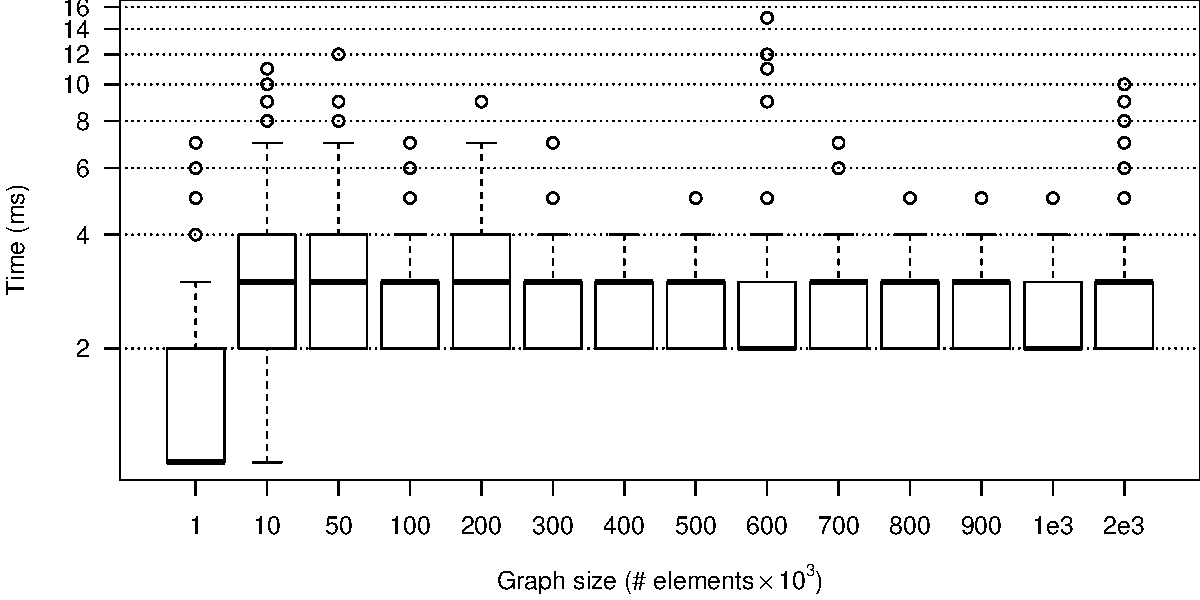
\includegraphics[width=0.85\linewidth]{img/chapt-tkm/validation/exp1-exec-log}
			\label{fig:exp1-exec}
	}
	\hfil
	\subfloat[Memory evolution] {
			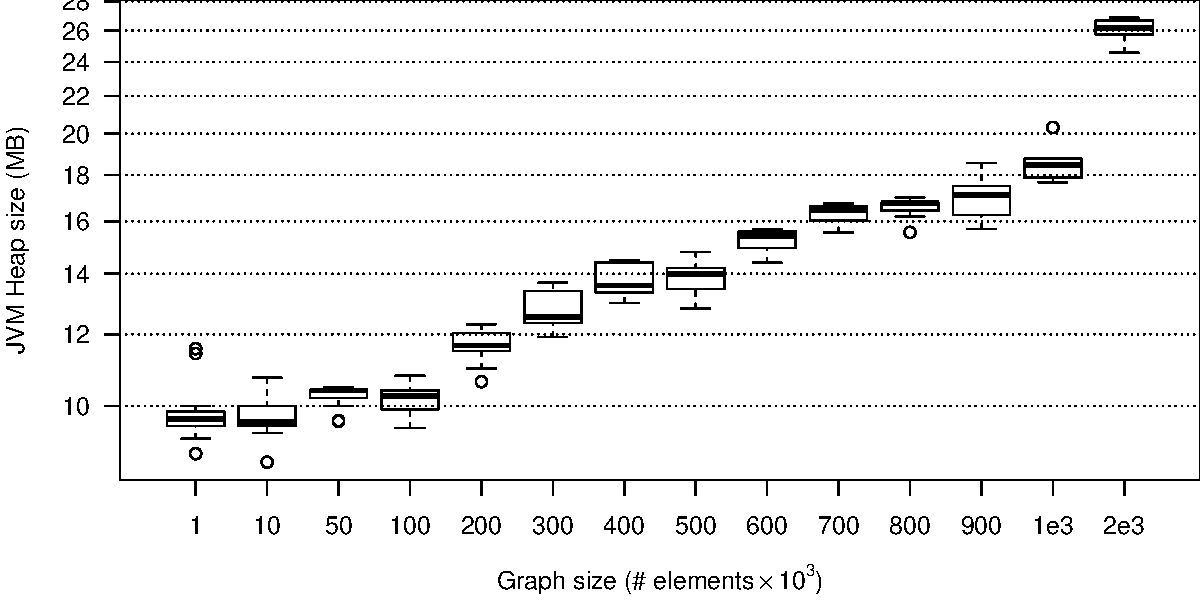
\includegraphics[width=0.85\linewidth]{img/chapt-tkm/validation/exp1-mem-log}
			\label{fig:exp1-mem}
		}	
	\caption{Experimentation results when the knowledge based size increases}
	\label{fig:exp1}
\end{figure}

\paragraph{How performance is influenced by the input size (I)?}
The second experiment aims to show the impact of the input size (I) on the execution of diagnosis algorithms. We fix the size of \textit{N} to 500\,000 and we variate \textit{I} from 1\,000 nodes to 100\,000, \ie from 0.2\% to 20\% of the graph size. 
The results are depicted in Figure~\ref{fig:exp-res} (straight lines).

Unlike to the previous experiment, we notice that the input size (\textit{I}) impacts the performance, both in terms of memory consumption and execution time. This is because our framework keeps in memory all the traversed elements, namely the input elements.
The increase in memory consumption follows a linear trend with regards to \textit{N}. As it can be noticed, it reaches 2GB for \textit{I}=100\,000. The execution time also shows a similar curve, while the query response time takes around than around 60ms to run for \textit{I}=1\,000, it takes a bit more than 4 seconds to finish for \textit{I}=100\,000. Nonetheless, these results remain very acceptable for diagnosis purposes. 

%The number of input elements is a clear scope of our approach.
%According to the results, our approach does not enable real-time diagnosis on very large scale models: with 100\,000 elements as input for an analysis, our approach requires around 4 seconds to extract all the data.
%However, our approach can be used for (near) real-time analysis for analysis that needs up to 1\,000 elements.
%Results show that for this size, our approach around 60 ms. 
%\begin{figure}
%	\centering
%	\subfigure[Execution time evolution]{
%		\includegraphics[width=0.47\linewidth]{img/exp2-exec}
%		\label{fig:exp2-exec}
%	}
%	\hfil
%	\subfigure[Memory evolution]{
%		\includegraphics[width=0.47\linewidth]{img/exp2-mem}
%		\label{fig:exp2-mem}
%	}
%	\caption{Memory and execution time behavior when the input size increases}
%	\label{fig:exp2}
%\end{figure}

\paragraph{How performance is influenced by the number of traversed elements (M)?}%

For the last experiment, we aim to highlight the impact of the number of traversed elements (\textit{M}). For this, we fix \textit{I} and \textit{O} to 1, and randomly generate a graph with sizes ranging from $1\,000$ to $100\,000$. Our algorithm navigates the whole model (\textit{M}=\textit{N}).
We depict the results in Figure~\ref{fig:exp-res} (dashed curve).
As we can notice, the memory consumption increases in a quasi-linear way. The memory footprint to traverse \textit{M} = 100\,000 elements is around 0.9GB. The progress of the execution time curve behaves similarly, in a quasi-linear way. Finally, the execution time of a full traversal over the biggest graph takes less than 2.5 seconds. 

%\begin{figure}
%	\centering
%	\subfigure[Execution time when the input size increases]{
%		\includegraphics[width=0.7\linewidth]{img/exp2-exec}
%		\label{fig:exp2-exec}
%	}
%	\hfil
%	\centering
%	\subfigure[Memory consumption when the input size increases]{
%		\includegraphics[width=0.7\linewidth]{img/exp2-mem}
%		\label{fig:exp2-mem}
%	}
%
%	\hfil
%	\centering
%	\subfigure[Execution time when the number of traversed elements increases]{
%		\includegraphics[width=0.7\linewidth]{img/exp4-exec}
%		\label{fig:exp4-exec}
%	}
%	\hfil
%	\centering
%	\subfigure[Memory consumption when the number of traversed elements increases]{
%		\includegraphics[width=0.7\linewidth]{img/exp4-mem}
%		\label{fig:exp4-mem}
%	}
%%	\caption{Memory and execution time behavior when the number of traversed elements increases}
%\caption{Results of experiments when the number of traversed or input elements  increases}
%%	\label{fig:exp4}
%\end{figure}

\begin{figure}
	\centering
	\subfloat[Evolution of the execution time]{
		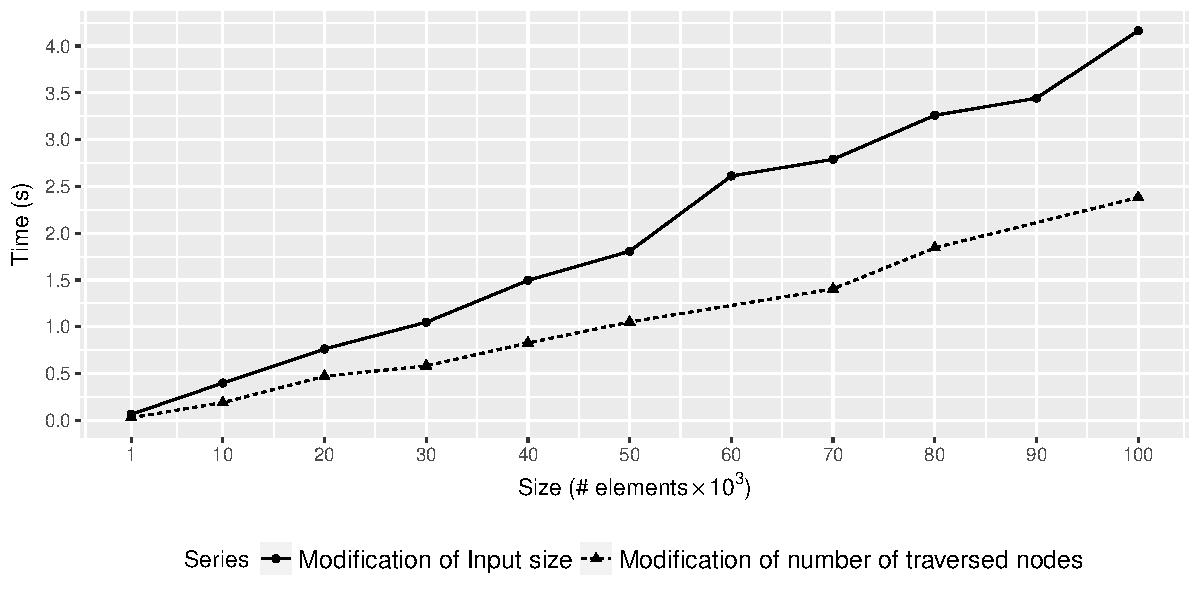
\includegraphics[width=0.9\linewidth]{img/chapt-tkm/validation/exp-exec}
		\label{fig:exp-exec}
	}
	\hfil
	\centering
	\subfloat[Evolution of the memory consumption]{
		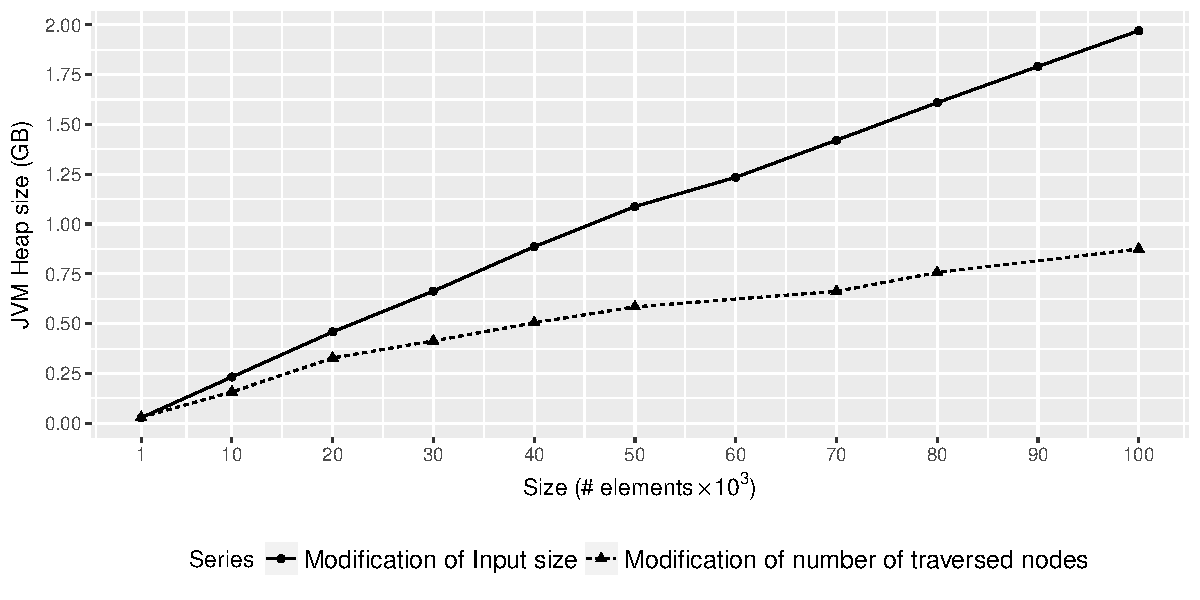
\includegraphics[width=0.9\linewidth]{img/chapt-tkm/validation/exp-mem}
		\label{fig:exp-mem}
	}
\caption{Results of experiments when the number of traversed or input elements  increases}
\label{fig:exp-res}
\end{figure}

\subsection{Discussion}
By linking context, actions, and requirements using decisions, data extraction for explanation or fault localization can be achieved by performing common temporal graph traversal operations.
In the detailed example, we show how a stakeholder could use our approach to define the different elements required by such systems, to structure runtime data, finally, to diagnose the behavior of adaptation processes. 
%In the three presented algorithms, we can see that these graph traversals allow us to navigate from action to goals, context to decisions and decisions to their circumstances and impact.
%By mixing these algorithms, we could also imagine a way to navigate from system states to decision circumstances and vice versa.

% By linking context, actions, and requirements using decisions, data extraction for explanation or fault localization can be achieved by performing common temporal graph traversal operations.
% In the detailed example, we show how a stakeholder could use our approach to define the different elements required by such systems, to structure runtime data and, finally, to diagnose the behavior adaptation process.

Our implementation allows to dynamically load and release nodes during the execution of a graph traversal. Using this feature, only the needed elements are kept in the main memory.  Hence, we can perform interactive diagnosis routines on large graphs with an acceptable memory footprint. 
However, the performance of our solution, in terms of memory and execution time, is restricted by the number of traversed elements and the number of input elements.
Indeed, as shown in our experimentation, both the execution time and the memory consumption grow linearly.

%As described in~\cite{DBLP:conf/smartgridcomm/0001FKTPTR14}, the smart grid in Luxembourg is composed of at most 88 elements (meters, data concentrators and central system included).
%The system generates from 120 to 623 updates per hour.
%100\,000 model elements correspond thus to the data of at least $\sim$7 days and at most $\sim$5 weeks.
%In other word, our approach can efficiently handle up to 1 month history data in $\sim$2.4s. \ab{explain where the numbers came from}
As described in~\cite{DBLP:conf/smartgridcomm/0001FKTPTR14}, the smart grid in Luxembourg is composed of 1 central system, 3 data concentrators and 227 meters.
The network is thus composed of 231 elements.
Each meter sends the consumption value every 15 min, being 908 every hours.
Plus, there is from 0 to 273 topology modifications in the network.
In total, the system generates from 908 to 1,181 new values every hour.
If we consider that we have one model element per smart grid entity and one model element per new value, 100,000 model elements correspond thus from $((100,000 - 231) * 1H ) / 1,181 = 84,5H$ ($\sim$ 3,5 days) to $((100,000 - 231) * 1H ) / 908 = 109,9H$ ($\sim$ 4,6 days) of data. In other word, our approach can efficiently interrogate up to $\sim$5 days history data in 2.4s.

%Over 100\,000 elements implied in a diagnosis process, we should distribute the models and the computation on different machines.
% Netflix infrastructure represents +100\,000 AWS instances and they have to manage 10\,000 starts per seconds\footnote{https://aws.amazon.com/solutions/case-studies/netflix/, Last visited: April 6th, 2018}.
% In average, 1 start require thus 10 instances. 
% If we consider that for each instance we model CPU, RAM and network data, then 1 start require $10 + (10 * 3) = 40$ model elements.
% 100\,000 elements correspond thus to $\sim$2,440 starts event with instances data.
% In $\sim$2.4s, our approach can extract data for $\sim$2,440 starts event, \ie 0.244s of Netflix start events.
% Our approach can navigate through data of start events for 1 day in more than 12 days.
% Even if our approach is suitable for small or medium adaptive systems, we can't use our approach on large adaptive systems for global diagnostics.
% A future work will consist in considering distributed adaptation systems to manage large ones.
